\section{Tích của véc-tơ với một số}

\subsection{Đề 1}
\Opensolutionfile{ans}[ans/ans-0-C4-B3-De1]
\caulc
%%%==============EX_10============%%%
\begin{ex}%[0H5H3-1]
Cho tam giác $ABC$. Gọi $I$ là trung điểm của $BC$. Khẳng định nào sau đây đúng?
	\choice
		{\True $\overrightarrow{BI}=\overrightarrow{IC}$}
		{$3\overrightarrow{BI}=2\overrightarrow{IC}$}
		{$\overrightarrow{BI}=\overrightarrow{2IC}$}
		{$\overrightarrow{2BI}=\overrightarrow{IC}$}
	\loigiai{
		Vì $I$ là trung điểm của $BC$ nên  $\overrightarrow{BI}=\overrightarrow{IC}$.
		}
\end{ex}

%%%==============EX_13============%%%
\begin{ex}%[0H5N3-4]
Cho ba điểm $A$, $B$, $C$ phân biệt. Điều kiện cần và đủ để ba điểm $A$, $B$, $C$  thẳng hàng là
	\choice
		{$AB=AC$}
		{\True $\exists k\ne 0$ sao cho $\overrightarrow{AB}=k\cdot \overrightarrow{AC}$}
		{$\overrightarrow{AC}-\overrightarrow{AB}=\overrightarrow{BC}$}
		{$\overrightarrow{MA}+\overrightarrow{MB}=3\overrightarrow{MC}$ với mọi điểm $M$}
	\loigiai{
		Điều kiện cần và đủ để ba điểm $A$, $B$, $C$  thẳng hàng là $\exists k\ne 0$ sao cho $\overrightarrow{AB}=k\cdot \overrightarrow{AC}$.
		}
\end{ex}
%%%==============EX_16============%%%
\begin{ex}%[0H5H3-2]
	\immini{
	Cho tam giác $ABC$ có trọng tâm $G$ và trung tuyến $AM$. Khẳng định nào sau đây \textbf{sai}?
	\choice
		{$\overrightarrow{GA}+\overrightarrow{GB}+\overrightarrow{GC}=\overrightarrow{0}$}
		{$\overrightarrow{GA}+2\overrightarrow{GM}=\overrightarrow{0}$}
		{\True $\overrightarrow{AM}=-2\overrightarrow{MG}$}
		{$\overrightarrow{OA}+\overrightarrow{OB}+\overrightarrow{OC}=3\overrightarrow{OG}$, với mọi điểm $O$}
		}{
		\begin{tikzpicture}[line join=round, line cap=round,thick,scale= 0.7]
				\coordinate (A) at (0,3);
				\coordinate (B) at (-2,0);
				\coordinate (C) at (3,0);
				\coordinate (M) at ($(B)!1/2!(C)$);
				\coordinate (G) at ($(A)!2/3!(M)$);
				\draw(A)--(B)--(C)--cycle;
				\draw(A)--(M) ;
				\foreach \i/\g in {A/90,B/-90,C/-90,M/-90,G/0}{\draw[fill=white](\i) circle (1pt) ($(\i)+(\g:3mm)$) node[scale=0.7]{$\i$};}
		\end{tikzpicture}
		}
	\loigiai{
		Ta có $\overrightarrow{AM}=-3\overrightarrow{MG}$.
		}
\end{ex}
%%%==============EX_17============%%%
\begin{ex}%[0H5H3-5]
	\immini{
	Cho tam giác $ABC$ có trung tuyến $AM$, khẳng định nào sau đây đúng?
	\choice
		{$\overrightarrow{AM}=\overrightarrow{AB}+2\overrightarrow{BM}$}
		{\True $\overrightarrow{AM}=\dfrac{1}{2} \left(\overrightarrow{AB}+\overrightarrow{AC}\right)$}
		{$\overrightarrow{AM}=-\dfrac{1}{2} \left(\overrightarrow{AB}+\overrightarrow{AC}\right)$}
		{$\overrightarrow{AM}=\dfrac{1}{2} \left(\overrightarrow{AB}-\overrightarrow{AC}\right)$}
		}{
		\begin{tikzpicture}[line join=round, line cap=round,thick,scale= 0.7]
				\coordinate (A) at (0,3);
				\coordinate (B) at (-2,0);
				\coordinate (C) at (3,0);
				\coordinate (M) at ($(B)!1/2!(C)$);
				\draw(A)--(B)--(C)--cycle;
				\draw(A)--(M) ;
				\foreach \i/\g in {A/90,B/-90,C/-90,M/-90}{\draw[fill=white](\i) circle (1pt) ($(\i)+(\g:3mm)$) node[scale=0.7]{$\i$};}
		\end{tikzpicture}
		}
	\loigiai{
		Theo tính chất trung điểm đoạn thẳng ta có $\overrightarrow{AB}+\overrightarrow{AC}=2\overrightarrow{AM}$.\\
		Suy ra $\overrightarrow{AM}=\dfrac{1}{2} \left(\overrightarrow{AB}+\overrightarrow{AC}\right)$.
		}
\end{ex}
%%%==============EX_18============%%%
\begin{ex}%[0H5H3-2]
	\immini{
	Cho hình bình hành $ABCD$ tâm $O$. Khẳng định nào sau đây đúng?
	\choice
		{$\overrightarrow{AB}+\overrightarrow{AD}=3\overrightarrow{AO}$}
		{\True $2\overrightarrow{AB}+3\overrightarrow{AC}+2\overrightarrow{AD}=5\overrightarrow{AC}$}
		{$\overrightarrow{AB}+\overrightarrow{AD}=2\overrightarrow{AC}$}
		{$\overrightarrow{AB}+\overrightarrow{AC}+\overrightarrow{AD}=2\overrightarrow{AO}$}
	}{
		\begin{tikzpicture}[scale=1, font=\footnotesize, line join=round, line cap=round, >=stealth]
				\path	(0,0) coordinate (A)++(0:3) coordinate (B)
				($(B)+(60:2)$) coordinate (C)
				($(A)+(C)-(B)$) coordinate (D)
				($(A)!1/2!(C)$)coordinate (O)
				;
				\draw (A)--(B)--(C)--(D)--(A)--(C) (B)--(D);
				\foreach \x/\g in {A/-150,B/-30,C/30,O/-90,D/100}  \fill (\x) circle (1.2pt)+(\g:.3)node {$\x$};	
		\end{tikzpicture}
	}
	\loigiai{
		Theo quy tắc hình bình hành $\overrightarrow{AB}+\overrightarrow{AD}=\overrightarrow{AC}$ nên
		\[2\overrightarrow{AB}+3\overrightarrow{AC}+2\overrightarrow{AD}=2\left(\overrightarrow{AB}+\overrightarrow{AD}\right)+3\overrightarrow{AC}=2\overrightarrow{AC}+3\overrightarrow{AC}=5\overrightarrow{AC}.
		\]
		}
\end{ex}


%%%==============EX_4============%%%
\begin{ex}%[0H5H3-2]
	\immini{
	Cho tam giác $ABC$. Gọi $M$, $N$, $P$ lần lượt là trung điểm của $BC$, $CA$, $AB$. Khẳng định nào sau đây \textbf{sai}?
	\choice
		{$\overrightarrow{MN}+\overrightarrow{NP}+\overrightarrow{PM}=\overrightarrow{0}$}
		{$\overrightarrow{PB}+\overrightarrow{MC}=\overrightarrow{PM}$}
		{\True $\overrightarrow{AB}+\overrightarrow{BC}+\overrightarrow{AC}=\overrightarrow{0}$}
		{$\overrightarrow{AP}+\overrightarrow{BM}+\overrightarrow{CN}=\overrightarrow{0}$}
		}{
		\begin{tikzpicture}[scale=1, font=\footnotesize, line join=round, line cap=round, >=stealth]
				\path	(0,0) coordinate (B)++(0:3) coordinate (C)
				($(B)+(60:2)$) coordinate (A)
				($(B)!1/2!(C)$)coordinate (M)
				($(A)!1/2!(C)$)coordinate (N)
				($(B)!1/2!(A)$)coordinate (P)
				;
				\draw (A)--(B)--(C)--(A) (A)--(M) (B)--(N) (C)--(P);
				\foreach \x/\g in {A/90,B/-150,C/0,M/-90, N/60, P/150}  \fill (\x) circle (1.2pt)+(\g:.3)node {$\x$};	
		\end{tikzpicture}
		}
	\loigiai{
		Ta có $\overrightarrow{AB}+\overrightarrow{BC}+\overrightarrow{AC}=2\overrightarrow{AC}\ne \overrightarrow{0}$.
		}
\end{ex}

%%%==============EX_9============%%%
\begin{ex}%[0H5H3-1]
	Cho ba điểm phân biệt $A,B,C$. Nếu $\overrightarrow{AB}=-3\overrightarrow{AC}$ thì đẳng thức nào dưới đây đúng?
	\choice
		{$\overrightarrow{BC}=-4\overrightarrow{AC}$}
		{$\overrightarrow{BC}=-2\overrightarrow{AC}$}
		{$\overrightarrow{BC}=2\overrightarrow{AC}$}
		{\True $\overrightarrow{BC}=4\overrightarrow{AC}$}
	\loigiai{
		Ta có $\overrightarrow{AB}=-3\overrightarrow{AC} \Rightarrow \vec{BA} = 3\vec{AC}$ .\\
		Do đó $\vec{BC} = \vec{BA} + \vec{AC} = 3\vec{AC}+\vec{AC} = 4\vec{AC}$.
		}
\end{ex}


%%%==============EX_12============%%%
\begin{ex}%[0H5H3-1]
	Cho hai véc-tơ $\overrightarrow{a}$, $\overrightarrow{b}$ ngược hướng và $\left|\overrightarrow{a}\right|=5,\left|\overrightarrow{b}\right|=15$. Với giá trị nào của $m$ thì $\overrightarrow{a}=m\overrightarrow{b}$?
	\choice
		{$m=3$}
		{\True $m=-\dfrac{1}{3}$}
		{$m=\dfrac{1}{3}$}
		{$m=-3$}
	\loigiai{
		Do $\overrightarrow{a},\overrightarrow{b}$ ngược hướng nên $m=-\dfrac{\left|\overrightarrow{a}\right|}{\left|\overrightarrow{b}\right|}=-\dfrac{5}{15}=-\dfrac{1}{3}$.
		}
\end{ex}
%%%==============EX_15============%%%
\begin{ex}%[0H5H3-2]
	\immini{
	Cho hình bình hành $ABCD$ có $M$ là giao điểm của hai đường chéo. Mệnh đề nào sau đây \textbf{sai}?
	\choice
		{$\overrightarrow{AB}+\overrightarrow{BC}=\overrightarrow{AC}$}
		{$\overrightarrow{AB}+\overrightarrow{AD}=\overrightarrow{AC}$}
		{$\overrightarrow{BA}+\overrightarrow{BC}=2 \overrightarrow{BM}$}
		{\True $\overrightarrow{MA}+\overrightarrow{MB}=\overrightarrow{MC}+\overrightarrow{MD}$}
		}{
		\begin{tikzpicture}[scale=1, font=\footnotesize, line join=round, line cap=round, >=stealth]
				\path	(0,0) coordinate (A)++(0:3) coordinate (B)
				($(B)+(60:2)$) coordinate (C)
				($(A)+(C)-(B)$) coordinate (D)
				($(A)!1/2!(C)$)coordinate (M)
				;
				\draw (A)--(B)--(C)--(D)--(A)--(C) (B)--(D);
				\foreach \x/\g in {A/-150,B/-30,C/30,M/-90,D/100}  \fill (\x) circle (1.2pt)+(\g:.3)node {$\x$};	
		\end{tikzpicture}
		}
	\loigiai{
		$\overrightarrow{MA}+\overrightarrow{MB}=\overrightarrow{MC}+\overrightarrow{MD}$ sai vì $\overrightarrow{MA}+\overrightarrow{MB}, \overrightarrow{MC}+\overrightarrow{MD}$ đối nhau.
		}
\end{ex}

%%%==============EX_23============%%%
\begin{ex}%[0H5H3-1]
Trên đường thẳng cho điểm $B$ nằm giữa hai điểm $A$ và $C$, với $AB=2a,AC=6a$. Đẳng thức nào sau đây đúng?
	\choice
		{\True $\overrightarrow{BC}=-2\overrightarrow{BA}$}
		{$\overrightarrow{BC}=-2\overrightarrow{AB}$}
		{$\overrightarrow{BC}=4\overrightarrow{AB}$}
		{$\overrightarrow{BC}=\overrightarrow{AB}$}
	\loigiai{
Có $AB=2a\Rightarrow BC=4a=2AB$.
		
Mà $\overrightarrow{BC};\overrightarrow{AB}$ cùng hướng nên $\overrightarrow{BC}=2\overrightarrow{AB}\Rightarrow \overrightarrow{BC}=-2\overrightarrow{BA}$.
		}
\end{ex}
%%%==============EX_24============%%%
\begin{ex}%[0H5H3-2]
	\immini{Cho hình chữ nhật $ABCD$. Gọi  $I$, $K$ lần lượt là trung điểm của $BC$ và $CD$. Khẳng định nào sau đây đúng?
	\choice
		{$\overrightarrow{AI}+\overrightarrow{AK}=2\overrightarrow{AC}$}
		{$\overrightarrow{AI}+\overrightarrow{AK}=\overrightarrow{AB}+\overrightarrow{AD}$}
		{$\overrightarrow{AI}+\overrightarrow{AK}=\overrightarrow{IK}$}
		{\True $\overrightarrow{AI}+\overrightarrow{AK}=\dfrac{3}{2} \overrightarrow{AC}$}
		}{
		\begin{tikzpicture}[line join=round, line cap=round,thick,scale= 0.7]
				\coordinate (A) at (0,0);
				\coordinate (B) at ($(A)+(90:2)$);
				\coordinate (D) at ($(A)+(0:3)$);
				\coordinate (C) at ($(B)+(D)-(A)$);
				\coordinate (I) at ($(B)!1/2!(C)$);
				\coordinate (K) at ($(C)!1/2!(D)$);
				\draw(A)--(B)--(C)--(D)--cycle;
				\draw(A)--(I) (A)--(K) ;
				\foreach \i/\g in {A/-120,B/120,C/60,D/-30,I/90,K/0}{\draw[fill=white](\i) circle (1pt) ($(\i)+(\g:3mm)$) node[scale=0.7]{$\i$};}
		\end{tikzpicture}
		}
	\loigiai{
	Ta có
		\[\overrightarrow{AI}+\overrightarrow{AK}=\dfrac{1}{2} \left(\overrightarrow{AB}+\overrightarrow{AC}\right)+\dfrac{1}{2} \left(\overrightarrow{AD}+\overrightarrow{AC}\right)=\overrightarrow{AC}+\dfrac{1}{2} \left(\overrightarrow{AB}+\overrightarrow{AD}\right)=\dfrac{3}{2} \overrightarrow{AC}.
		\]
		}
\end{ex}
%%%==============EX_26============%%%
\begin{ex}%[0H5V3-2]
	Cho tam giác $ABC$ đều tâm $O$; $M$ là điểm bất kì trong tam giác. Hình chiếu của $M$ xuống ba cạnh lần lượt là $D$, $E$, $F$. Hệ thức nào sau đây là đúng?
	\choice
		{$\overrightarrow{MD}+\overrightarrow{ME}+\overrightarrow{MF}=\dfrac{1}{2} \overrightarrow{MO}$}
		{$\overrightarrow{MD}+\overrightarrow{ME}+\overrightarrow{MF}=\dfrac{2}{3} \overrightarrow{MO}$}
		{$\overrightarrow{MD}+\overrightarrow{ME}+\overrightarrow{MF}=\dfrac{3}{4} \overrightarrow{MO}$}
		{\True $\overrightarrow{MD}+\overrightarrow{ME}+\overrightarrow{MF}=\dfrac{3}{2} \overrightarrow{MO}$}
	\loigiai{
\begin{center}
\begin{tikzpicture}[scale=0.8,>=stealth,line join=round,line cap=round,font=\footnotesize]
	\def\a{6}
	\path (0:0) coordinate (B)
			++(0:\a) coordinate (C)
			([turn]120:\a) coordinate (A)
			++(-100:\a/2) coordinate (M)
			($(B)!(M)!(C)$) coordinate (D)
			($(A)!(M)!(C)$) coordinate (E)
			($(A)!(M)!(B)$) coordinate (F)
			($(M)+(C)-(B)$) coordinate (X)
			($(M)+(A)-(B)$) coordinate (Y)
			($(M)+(A)-(C)$) coordinate (Z)
			(intersection of Y--M and A--C) coordinate (A_1)
			(intersection of Y--M and B--C) coordinate (B_1)
			(intersection of Z--M and A--B) coordinate (A_2)
			(intersection of Z--M and B--C) coordinate (C_1)
			(intersection of X--M and A--B) coordinate (B_2)
			(intersection of X--M and A--C) coordinate (C_2);
	\draw (A)--(B)--(C)--cycle	(B_1)--(A_1)	(A_2)--(C_1)	(B_2)--(C_2);
	\draw[dashed,thick] 	(M)--(D)	(M)--(E)	(M)--(F);
	\draw pic[draw,angle radius=2mm]{right angle=C--D--M};%Theo chiều dương
	\draw pic[draw,angle radius=2mm]{right angle=M--F--A};
	\draw pic[draw,angle radius=2mm]{right angle=A--E--M};
	\foreach \x/ \goc in {A/135,B/-135,C/-45,D/-90,E/0,F/160, A_1/0,B_1/-90,C_1/-90,A_2/160,B_2/160,C_2/0} 
			\fill (\x) circle (1.5pt)
			($(\x)+(\goc:3mm)$) node {$\x$};
	\foreach \x/ \goc in {M/-30} \fill (\x) circle (1.5pt)
			($(\x)+(\goc:4mm)$) node {$\x$};		
\end{tikzpicture}
\end{center}
		Qua $M$ kẻ các đường thẳng $A_1 B_1 \parallel AB,A_2 C_1 \parallel AC,B_2 C_2 \parallel BC$.\\
		Suy ra  $\Delta MB_1 C_1, \Delta MA_1 C_2, \Delta MA_2 B_2$ là các tam giác đều.\\
		Ta có $\overrightarrow{MD}=\dfrac{1}{2} \left(\overrightarrow{MB_1}+\overrightarrow{MC_1}\right),\overrightarrow{ME}=\dfrac{1}{2} \left(\overrightarrow{MA_1}+\overrightarrow{MC_2}\right),\overrightarrow{MF}=\dfrac{1}{2} \left(\overrightarrow{MB_2}+\overrightarrow{MA_2}\right)$.

Suy ra 
$$\begin{aligned}
 \overrightarrow{MD}+\overrightarrow{ME}+\overrightarrow{MF} &=\dfrac{1}{2} \left(\overrightarrow{MA_1}+\overrightarrow{MA_2}\right)+\dfrac{1}{2} \left(\overrightarrow{MB_1}+\overrightarrow{MB_2}\right)+\dfrac{1}{2} \left(\overrightarrow{MC_1}+\overrightarrow{MC_2}\right)\\
 &=\dfrac{1}{2} \left(\overrightarrow{MA}+\overrightarrow{MB}+\overrightarrow{MC}\right)=\dfrac{3}{2} \overrightarrow{MO}.
\end{aligned}$$
	}
\end{ex}

\Closesolutionfile{ans}
\indapan{6}{ans/ans-0-C4-B3-De1}
\cauds
\Opensolutionfile{ans}[ans/ans-0-C4-B3-De1-DS]

\begin{ex}%[0H5N3-2]
%Câu 1.
 Cho hình bình hành $ABCD$ và các điểm $M$, $N$, $P$ thoả mãn $\overrightarrow{AM}=\dfrac{1}{2}\overrightarrow{AB}$, $\overrightarrow{AN}=\dfrac{1}{6}\overrightarrow{AC}$, $\overrightarrow{AP}=\dfrac{1}{4}\overrightarrow{AD}$. Các mệnh đề sau đúng hay sai?
\choiceTF
{\True $\overrightarrow{AN}=\dfrac{1}{6}(\overrightarrow{AB}+\overrightarrow{AD})$}
{$\overrightarrow{MN}=\dfrac{1}{3}\overrightarrow{AB}+\dfrac{1}{6}\overrightarrow{AD}$}
{$\overrightarrow{MP}=\dfrac{1}{3}\overrightarrow{AD}-\dfrac{1}{2}\overrightarrow{AB}$}
{\True Ba điểm $M$, $N$, $P$ thẳng hàng}
\loigiai{
\immini{
\begin{itemchoice}
	\itemch Ta có $\overrightarrow{AN}=\dfrac{1}{6}\overrightarrow{AC}=\dfrac{1}{6}\left(\overrightarrow{AB}+\overrightarrow{AD}\right)$.\\
	Vậy mệnh đề đã cho đúng.
	\itemch Ta có $\overrightarrow{MN}=\overrightarrow{AN}-\overrightarrow{AM}=\dfrac{1}{6}(\overrightarrow{AB}+\overrightarrow{AD})-\dfrac{1}{2}\overrightarrow{AB}$\\
	$=-\dfrac{1}{3}\overrightarrow{AB}+\dfrac{1}{6}\overrightarrow{AD}$.\\
	Vậy mệnh đề đã cho sai.
	\itemch Ta có $\overrightarrow{MP}=\overrightarrow{AP}-\overrightarrow{AM}=\dfrac{1}{4}\overrightarrow{AD}-\dfrac{1}{2}\overrightarrow{AB}$.\\
	Vậy mệnh đề đã cho sai.
	\itemch	Ta có  $\overrightarrow{MN}=\dfrac{1}{6}(\overrightarrow{AD}-2\overrightarrow{AB})=\dfrac{2}{3}\overrightarrow{MP}$.\\
Suy ra $\overrightarrow{MN},\overrightarrow{MP}$ cùng phương. Suy ra ba điểm $M,N,P$ thẳng hàng.\\
	Vậy mệnh đề đã cho đúng.
\end{itemchoice}
}
{\begin{tikzpicture}[scale=0.8, font=\footnotesize, line join=round, line cap=round, >=stealth]
		\path	(0,0) coordinate (A)
				(4,0) coordinate (B)
				(3,-3) coordinate (C)
				(-1,-3)coordinate (D)
				($(A)!1/2!(B)$)coordinate (M)
				($(A)!1/4!(D)$)coordinate (P)
				($(A)!1/6!(C)$)coordinate (N)
				;
				\draw (A)--(B)--(C)--(D)--cycle (A)--(C) (M)--(P);
				\foreach \x/\g in {A/90,B/90,C/-90,D/-90,M/90,N/-90,P/170}  \fill (\x) circle (1.2pt)+(\g:.3)node {$\x$};	
		\end{tikzpicture}}
	}
\end{ex}
%-------------------------------------------------------
\begin{ex}%[0H5H3-2]
%Câu 6. 
Cho hình bình hành $ABCD$ có tâm $O,M$ là một điểm bất kỳ. Các mệnh đề sau đúng hay sai?
 \choiceTF
{\True $\overrightarrow{AB}+\overrightarrow{AD}=\overrightarrow{AC}$}
{\True $\overrightarrow{AB}+5\overrightarrow{AC}+\overrightarrow{AD}=6\overrightarrow{AC}$}
{$\overrightarrow{MA}+\overrightarrow{MB}+\overrightarrow{MC}+\overrightarrow{MD}=\overrightarrow{MO}$}
{\True $\overrightarrow{MA}+\overrightarrow{MB}+\overrightarrow{MC}+\overrightarrow{MD}=4\overrightarrow{MO}$}
\loigiai{
\begin{itemchoice}
			\itemch Theo quy tắc hình bình hành ta có $\overrightarrow{AB}+\overrightarrow{AD}=\overrightarrow{AC}$.
			\itemch Ta có $\overrightarrow{AB}+5\overrightarrow{AC}+\overrightarrow{AD}=(\overrightarrow{AB}+\overrightarrow{AD})+5\overrightarrow{AC}=\overrightarrow{AC}+5\overrightarrow{AC}=6\overrightarrow{AC}$.
			\itemch Ta có  
\begin{eqnarray*}
&&\overrightarrow{MA}+\overrightarrow{MB}+\overrightarrow{MC}+\overrightarrow{MD}\\
&=&\overrightarrow{MO}+\overrightarrow{OA}+\overrightarrow{MO}+\overrightarrow{OB}+\overrightarrow{MO}+\overrightarrow{OC}+\overrightarrow{MO}+\overrightarrow{OD}\\
&=&4\overrightarrow{MO}+(\overrightarrow{OA}+\overrightarrow{OC})+(\overrightarrow{OB}+\overrightarrow{OD})\\
&=&4\overrightarrow{MO}.
\end{eqnarray*}
			\itemch Ta có  
\begin{eqnarray*}
&&\overrightarrow{MA}+\overrightarrow{MB}+\overrightarrow{MC}+\overrightarrow{MD}\\
&=&\overrightarrow{MO}+\overrightarrow{OA}+\overrightarrow{MO}+\overrightarrow{OB}+\overrightarrow{MO}+\overrightarrow{OC}+\overrightarrow{MO}+\overrightarrow{OD}\\
&=&4\overrightarrow{MO}+(\overrightarrow{OA}+\overrightarrow{OC})+(\overrightarrow{OB}+\overrightarrow{OD})\\
&=&4\overrightarrow{MO}.
\end{eqnarray*}
		\end{itemchoice}}
\end{ex}
%-------------------------------------------------------
\begin{ex}%[0H5H3-2]
%Câu 9. 
Cho $\triangle ABC$ nội tiếp đường tròn tâm $O$, $H$ là trực tâm tam giác, $D$ là điểm đối xứng của $A$ qua $O$. Các mệnh đề sau đúng hay sai?
 \choiceTF
{\True $BD\parallel CH$}
{\True $CD\parallel BH$}
{$\overrightarrow{HA}+\overrightarrow{HB}+\overrightarrow{HC}=3\overrightarrow{HO}$}
{$\overrightarrow{OA}+\overrightarrow{OB}+\overrightarrow{OC}=3\overrightarrow{OH}$}
\loigiai{
\immini{
		\begin{itemchoice}
			\itemch $\triangle ABD$ nội tiếp đường tròn đường kính $AD$ nên $AB\perp BD$.\\
			Mặt khác $AB\perp CH$ nên $BD\parallel CH$. \hfill (1)
			\itemch $\triangle ACD$ nội tiếp đường tròn đường kính $AD$ nên $AC\perp CD$.\\
			Mặt khác $AC\perp BH$ nên $CD\parallel BH$. \hfill (2)
			\itemch Từ (1) và (2) suy ra $BDCH$ là hình bình hành.\\
Ta có  $\overrightarrow{HA}+\overrightarrow{HB}+\overrightarrow{HC}=\overrightarrow{HA}+\overrightarrow{HD}=2\overrightarrow{HO}$.
			\itemch Ta có  
\begin{eqnarray*}
&&\overrightarrow{OA}+\overrightarrow{OB}+\overrightarrow{OC}=\overrightarrow{OH}+\overrightarrow{HA}+\overrightarrow{OH}+\overrightarrow{HB}+\overrightarrow{OH}+\overrightarrow{HC}\\
&=&3\overrightarrow{OH}+(\overrightarrow{HA}+\overrightarrow{HB}+\overrightarrow{HC})=3\overrightarrow{OH}+2\overrightarrow{HO}=\overrightarrow{OH}.
\end{eqnarray*}
		\end{itemchoice}
}
{\begin{tikzpicture}[scale=1, font=\footnotesize, line join=round, line cap=round, >=stealth]
		\path	(2,0) coordinate (A)
				(-1,-3) coordinate (B)
				($(B)+(4,0)$) coordinate (C)
				($(B)!1/2!(C)$)coordinate (M)
				($(A)!2/3!(M)$)coordinate (G)
				($(B)!(A)!(C)$)coordinate (a')
				($(A)!(C)!(B)$)coordinate (c')
				($(A)!(B)!(C)$)coordinate (b') 
				(intersection of A--a' and B--b')coordinate (H)
				($(H)!2!(M)$)coordinate (D)
				($(A)!1/2!(D)$)coordinate (O)
				;
				\draw (O) let \p1=($(O)-(A)$) in circle ({veclen(\x1,\y1)});
				\draw (A)--(B)--(C)--cycle (D)--(A)(A)--(a') (B)--(b') (C)--(H) (B)--(D)--(C);
				\foreach \x/\g in {A/90,B/-150,C/-45,H/125,D/-80,O/145}  \fill (\x) circle (1.2pt)+(\g:.3)node {$\x$};
				\foreach \a/\b/\c in {A/a'/C,B/b'/C}{\draw pic[draw,angle radius=2mm] {right angle = \a--\b--\c};}
		\end{tikzpicture}}
}
\end{ex}
%-------------------------------------------------------

\begin{ex}%[0H5H3-2]
%Câu 11. 
Cho hình thang cân $ABCD$ có $AB\parallel CD$, $AB=2AD=2CD$, $E$ là trung điểm cạnh $AB$. Các mệnh đề sau đúng hay sai?
 \choiceTF
{\True $\overrightarrow{AB}=2\overrightarrow{DC}$}
{\True $\overrightarrow{CA}+\overrightarrow{CB}=2\overrightarrow{CE}$}
{\True $\overrightarrow{AD}=\overrightarrow{EC}$}
{$\overrightarrow{DE}=-\overrightarrow{CB}$}
\loigiai{
\immini{
	\begin{itemchoice}
			\itemch Ta có $\vec{AB}, \vec{DC}$ cùng hướng và $AB = 2DC$ nên $\vec{AB}=2 \vec{DC}$.
			\itemch $E$ là trung điểm $AB$ nên $\overrightarrow{CA}+\overrightarrow{CB}=2\overrightarrow{CE}$.
			\itemch Ta có  $AE=CD=\dfrac{1}{2}AB,AE\parallel CD$ nên $AECD$ là hình bình hành. Do đó $\overrightarrow{AD}=\overrightarrow{EC}$.
			\itemch Hoàn toàn tương tự, ta chứng minh được $BCDE$ là hình bình hành. Suy ra $\overrightarrow{DE}=\overrightarrow{CB}$.
	\end{itemchoice}
	}{
	\begin{tikzpicture}[scale=0.8, font=\footnotesize, line join=round, line cap=round, >=stealth]
		\path	(0,0) coordinate (A)
				(6,0) coordinate (B)
				($(A)!1/2!(B)$)coordinate (E)							($(B)!1!-60:(E)$)coordinate (C)
				($(A)!1!60:(E)$)coordinate (D)
				;
				\draw (A)--(B)--(C)--(D)--cycle (A)--(C)--(E)--(D) (B)--(D);
				\foreach \x/\g in {A/-90,B/-90,C/90,D/90,E/-90}  \fill (\x) circle (1.2pt)+(\g:.3)node {$\x$};	
		\end{tikzpicture}
	}
}
\end{ex}
%-------------------------------------------------------
\Closesolutionfile{ans}
\indapan{3}{ans/ans-0-C4-B3-De1-DS}


\Opensolutionfile{ans}[ans/ans-0-C4-B3-De1-KQ]
\caukq
%%%==============BT_1==============%%%
\begin{ex}%[0H5H3-6]
	Cho $\triangle ABC$ vuông tại $B$ có $\widehat{A}=30^{\circ}, AB = \sqrt{3}$. Gọi $I$ là trung điểm của $AC$. Giá trị của $\left|\overrightarrow{BA}+\overrightarrow{BC}\right|$ bằng bao nhiêu?
	\shortans{$2$}
	\loigiai{
		\immini{	
			Xét $\triangle ABC$ vuông tại $B$ có $\tan A=\dfrac{BC}{AB} \Rightarrow BC=AB\cdot \tan A=\sqrt{3} \tan 30^{\circ}=1$.\\	
			$AC=\sqrt{A B^2+BC^2}=\sqrt{3+1}=2$.\\	
			Suy ra $\left| \overrightarrow{BA}+\overrightarrow{BC}\right|=\left| 2 \overrightarrow{B I}\right|=2\left| \overrightarrow{B I}\right|=2 B I=2 \cdot \dfrac{AC}{2}=AC=2$.
		}{
			\begin{tikzpicture}[scale=1, font=\footnotesize, line join=round, line cap=round, >=stealth]
				\path	(0,0) coordinate (B)++(0:3.46) coordinate (A)
				($(B)+(90:2)$) coordinate (C)
				($(A)!1/2!(C)$)coordinate (I)
				;
				\draw (A)--(B)--(C)--(A) (B)--(I);
				\foreach \x/\g in {A/0,B/-150,C/90,I/60}  \fill (\x) circle (1.2pt)+(\g:.3)node {$\x$};	
			\end{tikzpicture}
		}
	}
\end{ex}

%%%==============BT_3==============%%%
\begin{ex}%[0H5H3-6]
	Cho tứ giác $ABCD$. Gọi $I$, $J$ theo thứ tự là trung điểm của $AB$, $CD$ và $IJ=\dfrac{5}{4}$.	Gọi $M, N$ theo thứ tự là trung điểm của $BC, AC$. Giá trị của $\left|\overrightarrow{AM}+\overrightarrow{BN}+\overrightarrow{CJ}\right|$ bằng bao nhiêu?	
	\shortans{$1{,}25$}
	\loigiai{
		\immini{	
			Theo tính chất trung điểm ta có 	$\heva{ & 2 \overrightarrow{AM}=\overrightarrow{AB}+\overrightarrow{AC} \\
				& 2 \overrightarrow{BN}=\overrightarrow{B A}+\overrightarrow{BC}\\
				& 2\overrightarrow{CI}=\overrightarrow{CA}+\overrightarrow{CB}.
			}$\\
			Cộng ba đẳng thức trên ta được	\\
			$ 
			2\left(\overrightarrow{AM}+\overrightarrow{B N}+\overrightarrow{C I}\right)$\\
			$=\left(\overrightarrow{AB}+\overrightarrow{B A}\right)+\left(\overrightarrow{AC}+\overrightarrow{C A}\right)+\left(\overrightarrow{BC}+\overrightarrow{C B}\right)$\\
			$=\overrightarrow{0}.$	
			Suy ra $\overrightarrow{AM}+\overrightarrow{BN}+\overrightarrow{CJ} = \overrightarrow{AM}+\overrightarrow{BN}+\overrightarrow{CI} + \overrightarrow{IJ}=\overrightarrow{0} +\overrightarrow{IJ} = \vec{IJ}$.\\
			Do vậy $\left|\overrightarrow{AM}+\overrightarrow{BN}+\overrightarrow{CJ}\right|=\left|\vec{IJ}\right| = \dfrac{5}{4}$.
		}{
			\begin{tikzpicture}[scale=0.8, font=\footnotesize, line join=round, line cap=round, >=stealth]
				\path	(0,0) coordinate (A)++(0:4) coordinate (B)++(120:4) coordinate (C)++(-150:2) coordinate (D)
				($(B)!1/2!(A)$)coordinate (I)
				($(C)!1/2!(D)$)coordinate (J)
				($(C)!1/2!(B)$)coordinate (M)
				($(C)!1/2!(A)$)coordinate (N)
				;
				\draw (A)--(B)--(C)--(D)--(A)--(C) (A)--(M) (B)--(N) (C)--(I);
				\foreach \x/\g in {A/-150,B/-20,C/90,D/120,I/-90,J/120,M/10,N/160}  \fill (\x) circle (1.2pt)+(\g:.3)node {$\x$};	
			\end{tikzpicture}
		}
	}
\end{ex}

%%%==============BT_5==============%%%
\begin{ex}%[0H5V3-9]
	\immini{
		Một chất điểm $A$ chịu tác dụng của ba lực $\overrightarrow{F_1}, \overrightarrow{F_2}, \overrightarrow{F_3}$ như hình vẽ biết chất điểm $A$ đang ở trạng thái cân bằng. Nếu độ lớn của lực $\vec{F}_1$ bằng $12$(N)  thì độ lớn của lực $F_3$ bằng bao nhiêu (làm tròn kết quả đến hàng phần mười theo đơn vị N)?
	}{
		\begin{tikzpicture}[rotate=90,scale=1.3, font=\footnotesize, line join=round, line cap=round, >=stealth]
			\path	(0,0) coordinate (A)++(0:1) coordinate (y)
			($(A)+(-90:1.73)$) coordinate (x)
			($(A)+(120:2)$) coordinate (z)
			($(A)!0.8!(x)$) coordinate (F1) node[above,scale =1]{$\vec{F_1}$}
			($(A)!0.8!(y)$) coordinate (F2) node[right,scale =1]{$\vec{F_2}$}
			($(A)!0.8!(z)$) coordinate (F3) node[above left,scale =1]{$\vec{F_3}$}
			;
			\draw[thick,->] (A)--(x);
			\draw[thick,->] (A)--(y);
			\draw[thick,->] (A)--(z);
			\pic[draw,thin,angle radius=2mm] {right angle = y--A--x};
			\pic[draw,thin,angle radius=2mm] {angle = y--A--z};
			\foreach \x/\g in {A/-180}  \fill (\x) circle (1.2pt)+(\g:.3)node {$\x$};
			\foreach \x/\g in {A/60}  \fill (\x) circle (1.2pt)+(\g:.4)node {$120$};	
		\end{tikzpicture}
	}
	\shortans{$13{,}9$}
	\loigiai{
		\immini{	
			Đặt $\vec{F}_1=\overrightarrow{AB}, \overrightarrow{F_2}=\overrightarrow{AD}, \overrightarrow{F_3}=\overrightarrow{AE}$.\\
			Dựng hình chữ nhật $A BC D$. Do vật ở trạng thái cân bằng nên	
			\[
			\vec{F}_1+\vec{F}_2+\overrightarrow{F_3}=\overrightarrow{0} \Leftrightarrow \overrightarrow{AB}+\overrightarrow{AD}+\overrightarrow{A E}=\overrightarrow{0} \Leftrightarrow \overrightarrow{AC}=-\overrightarrow{A E}.
			\]	
			Ta có $A B=12, \widehat{C AD}=180^{\circ}-120^{\circ}=60^{\circ} \Rightarrow  \widehat{B AC}=30^{\circ}$.
		}{
			\begin{tikzpicture}[rotate=90,scale=1.3, font=\footnotesize, line join=round, line cap=round, >=stealth]
				\path	(0,0) coordinate (A)++(0:1) coordinate (D)
				($(A)+(120:2)$) coordinate (E)
				($(A)+(-60:2)$) coordinate (C)
				($(A)+(C)-(D)$) coordinate (B)
				;
				\draw (A)--(B) (A)--(D) (A)--(E) (A)--(C) (B)--(C)--(D);
				\pic[draw,thin,angle radius=2mm] {right angle = D--A--B};
				\pic[draw,thin,angle radius=2mm] {angle = D--A--E};
				\foreach \x/\g in {A/-180,D/30,C/-30,B/-120,E/0}  \fill (\x) circle (1.2pt)+(\g:.2)node {$\x$};	
				\foreach \x/\g in {A/60}  \fill (\x) circle (1.2pt)+(\g:.4)node {$120$};
			\end{tikzpicture}
		}
		\noindent		
		Tam giác $A BC$ vuông tại $B$ nên $BC=A B \tan 30^{\circ}=12 \cdot \dfrac{\sqrt{3}}{3}=4 \sqrt{3}=AD$.\\
		Suy ra $AC=\sqrt{A B^2+BC^2}=\sqrt{12^2+(4 \sqrt{3})^2}=8 \sqrt{3}$. Do vậy $\left|\overrightarrow{F_3}\right|=\left|\overrightarrow{A E}\right|=AC=8\sqrt{3} \approx 13{,}9$.
	}
\end{ex}

%%%==============BT_6==============%%%
\begin{ex}%[0H5H3-5]
	Cho tam giác $ABC$. Gọi $M$ là một điểm trên cạnh $BC$ sao cho $MB=2MC$. Nếu $\overrightarrow{AM} = m\overrightarrow{AB} + n \overrightarrow{AC}$ thì giá trị của $3m - 3n$ bằng bao nhiêu?	
	\shortans{$-1$}	
	\loigiai{
		\immini{	
			Ta có
			\[ 
			\overrightarrow{AM}=\overrightarrow{AC}+\overrightarrow{C M}=\overrightarrow{AC}-\dfrac{1}{3} \overrightarrow{BC} =\overrightarrow{AC}-\dfrac{1}{3}\left(\overrightarrow{AC}-\overrightarrow{AB}\right)=\dfrac{1}{3} \overrightarrow{AB}+\dfrac{2}{3} \overrightarrow{AC}.
			\]
			Suy ra $m = \dfrac{1}{3}$, $n = \dfrac{2}{3}\Rightarrow 3m -3n = -1$.
		}{
			\begin{tikzpicture}[scale=1, font=\footnotesize, line join=round, line cap=round, >=stealth]
				\path	(0,0) coordinate (B)++(0:3) coordinate (C)
				($(B)+(60:2)$) coordinate (A)
				($(B)!2/3!(C)$)coordinate (M)
				;
				\draw (A)--(B)--(C)--(A) (A)--(M);
				\foreach \x/\g in {A/90,B/-150,C/0,M/-90}  \fill (\x) circle (1.2pt)+(\g:.3)node {$\x$};	
			\end{tikzpicture}
		}
	}
\end{ex}

%%%==============BT_12==============%%%
\begin{ex}%[0H5H3-5]
	Cho hình bình hành $ABCD$. Gọi $E$ và $F$ là $2$ điểm thỏa $\overrightarrow{BE}=\dfrac{1}{3}$, $\overrightarrow{BC}, \overrightarrow{BF}=\dfrac{1}{4} \overrightarrow{BD}$. Khi đó $\overrightarrow{AE}=k\overrightarrow{AF}$. Vậy giá trị $k$ bằng bao nhiêu (kết quả làm tròn đến hàng phần trăm)?
	\shortans{$1{,}33$}
	\loigiai{\immini{
			Ta phân tích $\overrightarrow{AE}$ và $\overrightarrow{AF}$ theo $2$ véc-tơ $\overrightarrow{AB}$ và $\overrightarrow{AD}$.\\
			Ta có $\overrightarrow{AE}=\overrightarrow{AB}+\overrightarrow{BE}=\overrightarrow{AB}+\dfrac{1}{3} \overrightarrow{BC}=\overrightarrow{AB}+\dfrac{1}{3} \overrightarrow{AD}$. \\
			Mặt khác $\overrightarrow{AF}=\overrightarrow{AB}+\overrightarrow{BF}=\overrightarrow{AB}+\dfrac{1}{4}\left(\overrightarrow{AD}-\overrightarrow{AB}\right)=\dfrac{3}{4} \overrightarrow{AB}+\dfrac{1}{4} \overrightarrow{AD}$.
		}
		{	\begin{tikzpicture}[scale=0.8, font=\footnotesize, line join=round, line cap=round, >=stealth]
				\coordinate (A) at (1,3);
				\coordinate (B) at (6,3);
				\coordinate (D) at (0,0);
				\coordinate (C) at ($(B)+(D)-(A)$);
				\coordinate (E) at ($(B)!1/3!(C)$);
				\coordinate (F) at ($(B)!1/4!(D)$);
				\draw(A)--(B)--(C)--(D)--cycle;
				\draw(A)--(E) (B)--(D);
				\foreach \i/\g in {A/90,B/90,C/-90,D/-90,E/0,F/90}{\draw[fill=black](\i) circle (1.5pt) ($(\i)+(\g:3mm)$) node[scale=1]{$\i$};}
			\end{tikzpicture}
		}
		
Xét hệ $\heva{&\overrightarrow{AE} = \overrightarrow{AB } + \dfrac {1}{3} \overrightarrow{AD} \\ &\overrightarrow{AF} = \dfrac {3}{4} \overrightarrow{AB}+ \dfrac{1}{4} \overrightarrow{AD}} \Leftrightarrow \heva{&\overrightarrow{AE}=\overrightarrow{AB}+\dfrac{1}{3} \overrightarrow{AD} \\ &\dfrac{4}{3} \overrightarrow{AF}=\overrightarrow{AB}+\dfrac{1}{3} \overrightarrow{AD}} \Leftrightarrow \overrightarrow{AE}=\dfrac{4}{3} \overrightarrow{AF}$.
	}
\end{ex}
%%%==============BT_13==============%%%
\begin{ex}%[0H5H3-5]
	Cho hình bình hành $ABCD$ tâm $O$. Lấy các điểm $I$, $J$ sao cho $3\overrightarrow{IA}+2 \overrightarrow{IC}-2 \overrightarrow{ID}=\overrightarrow{0}$, $\overrightarrow{JA}-2 \overrightarrow{JB}+2\overrightarrow{JC}=\overrightarrow{0}$. Nếu $\overrightarrow{IJ}=k \overrightarrow{IO}$ thì giá trị của $k$ bằng bao nhiêu?\par
	\shortans{$4$}
	\loigiai
	{
		Theo đề ta có
		\begin{eqnarray*}
			& & 3 \overrightarrow{IA}+2 \overrightarrow{IC}-2 \overrightarrow{ID}=\overrightarrow{0}\Leftrightarrow  3 \overrightarrow{IA}+2(\overrightarrow{IC}-\overrightarrow{ID})=\overrightarrow{0}\\
			&\Leftrightarrow & 3 \overrightarrow{IA}+2 \overrightarrow{DC}=\overrightarrow{0}\Leftrightarrow 3 \overrightarrow{IA}+2 \overrightarrow{AB}=\overrightarrow{0}\Leftrightarrow \overrightarrow{AI}=\dfrac{2}{3} \overrightarrow{AB}
		\end{eqnarray*}
		Mặt khác $\overrightarrow{JA}-2 \overrightarrow{JB}+2 \overrightarrow{JC}=\overrightarrow{0} \Leftrightarrow \overrightarrow{AJ}+2\left(\overrightarrow{JC}-\overrightarrow{JB}\right)=\overrightarrow{0} \Leftrightarrow \overrightarrow{AJ}=2\overrightarrow{BC} \Leftrightarrow \overrightarrow{AJ}=2 \overrightarrow{AD}$.\\
		Ta có $\overrightarrow{IO}=\overrightarrow{AO}-\overrightarrow{AI}=\dfrac{1}{2} \overrightarrow{AC}-\dfrac{2}{3} \overrightarrow{AB}=\dfrac{1}{2}\left(\overrightarrow{AB}+\overrightarrow{AD}\right)-\dfrac{2}{3} \overrightarrow{AB}=-\dfrac{1}{6} \overrightarrow{AB}+\dfrac{1}{2} \overrightarrow{AD}$\\
		và $\overrightarrow{IJ}=\overrightarrow{AJ}-\overrightarrow{AI}=2\overrightarrow{AD}-\dfrac{2}{3} \overrightarrow{AB}=-\dfrac{2}{3}\overrightarrow{AB}+2 \overrightarrow{AD}$.\\
		Do đó $\heva{&\overrightarrow{IO} = - \dfrac{1}{6} \overrightarrow{AB} + \dfrac{1}{2} \overrightarrow{AD} \\ &\overrightarrow{IJ} = - \dfrac {2}{3} \overrightarrow{AB} + 2 \overrightarrow{AD}} \Leftrightarrow \heva{&6 \overrightarrow{IO}=-\overrightarrow{AB}+3 \overrightarrow{AD}\\&\dfrac{3}{2} \overrightarrow{IJ}=-\overrightarrow{AB}+3 \overrightarrow{A D}}\Rightarrow 6 \overrightarrow{IO}=\dfrac{3}{2} \overrightarrow{IJ} \Leftrightarrow \overrightarrow{IJ}=4 \overrightarrow{IO}$.
	}
\end{ex}

\Closesolutionfile{ans}
\indapan{6}{ans/ans-0-C4-B3-De1-KQ}
\newpage 
\subsection{Đề 2}

\Opensolutionfile{ans}[ans/ans-0-B1]
\caulc
%%%==============EX_27============%%%
\begin{ex}%[text tai lieu Duong Hung, Huỳnh Xuân Tín]%[0H5V3-6]
	Cho tam giác đều $ABC$. Phát biểu nào sau đây đúng?
	\choice
	{$\overrightarrow{AB}-\overrightarrow{BC}=\overrightarrow0$}
	{\True $\left|\overrightarrow{AB}\right|=\left|\overrightarrow{AC}\right|$}
	{$\overrightarrow{AB}=\overrightarrow{AC}$}
	{$\overrightarrow{AB}+\overrightarrow{BC}=\overrightarrow{CA}$}
	\loigiai{
		Vì $\triangle ABC$ đều nên $AB=AC\Rightarrow \left|\overrightarrow{AB}\right|=\left|\overrightarrow{AC}\right|$.
	}
\end{ex}
%%%==============EX_28============%%%
\begin{ex}%[text tai lieu Duong Hung, Huỳnh Xuân Tín]%[0H5V3-6]
	Cho tam giác $ABC$, có bao nhiêu điểm $M$ thỏa $\left|\overrightarrow{MA}+\overrightarrow{MB}+\overrightarrow{MC}\right|=5$?
	\choice
	{$1$}
	{$2$}
	{\True Vô số}
	{Không có điểm nào}
	\loigiai{
		Gọi $G$ là trọng tâm tam giác $ABC$, ta có:
		$$\left|\overrightarrow{MA}+\overrightarrow{MB}+\overrightarrow{MC}\right|=5\Leftrightarrow \left|3\overrightarrow{MG}\right|=5\Leftrightarrow MG=\dfrac{5}{3}
		$$
		Vậy quỹ tích điểm $M$ là đường tròn tâm $G$, bán kính $\dfrac{5}{3}$.
	}
\end{ex}
%%%==============EX_29============%%%
\begin{ex}%[text tai lieu Duong Hung, Huỳnh Xuân Tín]%[0H5V3-6]
	Trên trục tọa độ $\left(O; \overrightarrow{e}\right)$, các điểm $A, B$ và $C$ có tọa độ lần lượt là $-1$; $2$ và $3$. Tìm giá trị của $\overline{AB}+2\overline{AC}$.
	\choice
	{\True $11$}
	{$1$}
	{$7$}
	{$-11$}
	\loigiai{
		\[\overline{AB}=2-\left(-1\right)=3, \overline{AC}=3-\left(-1\right)=4\Rightarrow \overline{AB}+2\overline{AC}=3+2\cdot4=11.
		\]
	}
\end{ex}
%%%==============EX_30============%%%
\begin{ex}%[text tai lieu Duong Hung, Huỳnh Xuân Tín]%[0H5V3-6]
	Cho hình chữ nhật $ABCD$ có $AB=4a$ và $AD=3a$. Độ dài của vecto $\overrightarrow{BA}+\overrightarrow{DA}$ bằng
	\choice
	{\True $5a$}
	{$6a$}
	{$2a\sqrt{3}$}
	{$7a$}
	\loigiai{
	\immini{Từ $B$ kẻ $\overrightarrow{BE}=\overrightarrow{DA}$.\\
		Áp dụng quy tắc hình hình hành: $\overrightarrow{BA}+\overrightarrow{DA}=\overrightarrow{BA}+\overrightarrow{BE}=\overrightarrow{BF}$ (với $F$ là đỉnh thứ tư của hình chữ nhật $ABEF$).\\
Vậy $\left|\overrightarrow{BF}\right|=\sqrt{(4a)^2+(3a)^2}=5a.
		$}{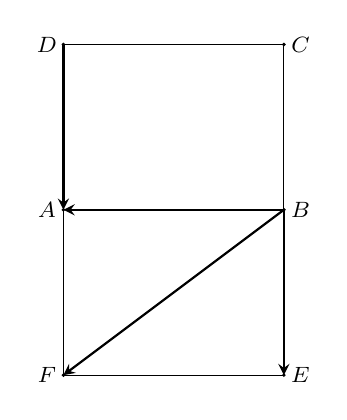
\begin{tikzpicture}[scale=0.7, font=\footnotesize, line join=round, line cap=round, >=stealth]
			\path	(0,0) coordinate (A)
			(4,0) coordinate (B)
		(0,3) coordinate (D)	
		(4,3) coordinate (C)
		(4,-3) coordinate (E)
		(0,-3) coordinate (F);
			\draw[thick,->] (B)--(A);
			\draw[thick,->] (D)--(A);
			\draw[thick,->] (B)--(E);
			\draw[thick,->] (B)--(F);
			\draw (E)--(F)--(A) (D)--(C)--(B);
			\foreach \x/\g in {A/180,D/180,F/180,E/0,B/0,C/0}  \fill (\x) circle (1.0pt)+(\g:.3)node {$\x$};	
	\end{tikzpicture}}	
	}
\end{ex}

%%%==============EX_31============%%%
\begin{ex}%[text tai lieu Duong Hung, Huỳnh Xuân Tín]%[0H5V3-6]
	Cho tam giác đều $ABC$ cạnh bằng $2a$. Khi đó $\left|\overrightarrow{AB}+\overrightarrow{AC}\right|$ bằng
	\choice
	{$a$}
	{\True $2\sqrt{3} a$}
	{$\dfrac{\sqrt{3} a}{2}$}
	{$2a$}
	\loigiai{
		\immini{	Ta có $\left|\overrightarrow{AB}+\overrightarrow{AC}\right|=\left|2\overrightarrow{AM}\right|=2.\dfrac{\sqrt{3}}{2}.2a=2\sqrt{3} a$.\\
		(với $M$ là trung điểm $BC$)}{\begin{tikzpicture}[scale=0.7, font=\footnotesize, line join=round, line cap=round, >=stealth]
				\path	(0,0) coordinate (A)
				(0:4) coordinate (B)
				(60:4) coordinate (C)	
	 ($(C)!0.5!(B)$) coordinate (M);
				\draw[thick,->] (A)--(B);
				\draw[thick,->] (A)--(C);
				\draw[thick,->] (A)--(M);
				\draw (B)--(C);
				\foreach \x/\g in {A/180,M/60,B/0,C/90}  \fill (\x) circle (1.0pt)+(\g:.3)node {$\x$};	
		\end{tikzpicture}}	
	}
\end{ex}
%%%==============EX_32============%%%
\begin{ex}%[text tai lieu Duong Hung, Huỳnh Xuân Tín]%[0H5V3-6]
Cho hình bình hành $ABCD$ có $AB=a$, $AB\bot BD$, $\widehat{BAD}=60^\circ$. Gọi $E$, $F$ lần lượt là trung điểm của $BD$, $AD$. Độ dài của véc-tơ $\overrightarrow{BE}+\overrightarrow{AF}$ là
	\choice
	{\True $\dfrac{a\sqrt{13}}{2}$}
	{$\dfrac{a\sqrt{10}}{2}$}
	{$\dfrac{a\sqrt{7}}{2}$}
	{$2a$}
	\loigiai{
			\immini{	Ta có $BD=a\cdot\tan 60^o=a\sqrt{3}$.\\ $GD=\sqrt{BD^2+BG^2}=\sqrt{\dfrac{a^2}{4}+3a^2}=\dfrac{a\sqrt{13}}{2}$.\\
			$\overrightarrow{BE}+\overrightarrow{AF}=-(\overrightarrow{DE}+\overrightarrow{DF})=-2\overrightarrow{DH}=-\overrightarrow{DG}$.\\
Do đó $\left|\overrightarrow{BE}+\overrightarrow{AF}\right|=DG=\dfrac{a\sqrt{13}}{2}.
				$}{\begin{tikzpicture}[scale=0.7, font=\footnotesize, line join=round, line cap=round, >=stealth]
				\path	(0,0) coordinate (A)
				(0:4) coordinate (B)
				(-60:8) coordinate (D)			
	 ($(B)+(D)-(A)$) coordinate (C)		
				($(D)!0.5!(B)$) coordinate (E)
($(D)!0.5!(A)$) coordinate (F)	($(A)!0.5!(B)$) coordinate (G) ($(E)!0.5!(F)$) coordinate (H)			;
				\draw[thick,->] (B)--(E);
				\draw[thick,->] (A)--(F);
				\draw (A)--(B)--(C)--(D)--(F)--(E)--(D)--(G);
				\foreach \x/\g in {A/90,E/0,F/-150,B/90,C/0,G/90,H/70}  \fill (\x) circle (1.0pt)+(\g:.3)node {$\x$};	
		\end{tikzpicture}}	
	}
\end{ex}
%%%==============EX_33============%%%
\begin{ex}%[text tai lieu Duong Hung, Huỳnh Xuân Tín]%[0H5V3-6]
	Cho tam giác $ABC$ vuông cân tại $A$, $AB=a$. Tính độ dài véc-tơ $\overrightarrow{AB}+4\overrightarrow{AC}$.
	\choice
	{$\sqrt{20} a$}
	{$5a$}
	{$17a$}
	{\True $\sqrt{17} a$}
	\loigiai{
		\immini{	Dựng các điểm $D$, $E$ sao cho $\overrightarrow{AD}=4\overrightarrow{AC}$ và tứ giác $ABED$ là hình bình hành.\\
			Khi đó $\left|\overrightarrow{AB}+4\overrightarrow{AC}\right|=\left|\overrightarrow{AB}+\overrightarrow{AD}\right|=\left|\overrightarrow{AE}\right|$.\\
			Áp dụng định lý Pi-ta-go cho tam giác $ADE$ ta có\\
		$\left|\overrightarrow{AB}+4\overrightarrow{AC}\right|=\sqrt{a^2+(4a)^2}=a\sqrt{17}$.	}{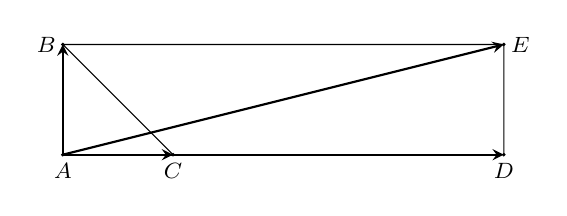
\begin{tikzpicture}[scale=0.7, font=\footnotesize, line join=round, line cap=round, >=stealth]
				\path	(0,0) coordinate (A)
				(0:2) coordinate (C)
				(90:2) coordinate (B)			
				(8,0) coordinate (D)		
				(8,2) coordinate (E)		;
				\draw[thick,->] (A)--(B);
				\draw[thick,->] (A)--(C);
				\draw[thick,->] (A)--(D);
				\draw[thick,->] (A)--(E);
				\draw (C)--(B)--(E)--(D);
				\foreach \x/\g in {A/-90,E/0,B/180,C/-90,D/-90}  \fill (\x) circle (1.0pt)+(\g:.3)node {$\x$};	
		\end{tikzpicture}}	
	}
\end{ex}
%%%==============EX_34============%%%
\begin{ex}%[text tai lieu Duong Hung, Huỳnh Xuân Tín]%[0H5V3-6]
	Cho tam giác $ABC$ đều cạnh bằng $1$. Ta có
	\choice
	{\True $\left|\overrightarrow{AB}-\overrightarrow{CA}\right|=\sqrt{3}$}
	{$\left|\overrightarrow{AB}-\overrightarrow{CA}\right|=0$}
	{$\left|\overrightarrow{AB}-\overrightarrow{CA}\right|=2$}
	{$\left|\overrightarrow{AB}-\overrightarrow{AC}\right|=0$}
	\loigiai{
			\immini{Gọi $M$ là trung điểm của $BC$ ta có $AM=\dfrac{\sqrt{3}}{2}$. Khi đó $\overrightarrow{AB}-\overrightarrow{CA}=\overrightarrow{AB}+\overrightarrow{AC}=2\overrightarrow{AM}$.\\
				Nên $\left|\overrightarrow{AB}-\overrightarrow{CA}\right|=\left|\overrightarrow{AB}+\overrightarrow{AC}\right|=2\left|\overrightarrow{AM}\right|=\sqrt{3}$.}{\begin{tikzpicture}[scale=0.7, font=\footnotesize, line join=round, line cap=round, >=stealth]
				\path	(0,0) coordinate (A)
				(0:4) coordinate (B)
				(60:4) coordinate (C)	
				($(C)!0.5!(B)$) coordinate (M);
				\draw[thick,->] (A)--(B);
				\draw[thick,->] (C)--(A);
				\draw[thick,->] (A)--(M);
				\draw (B)--(C);
				\foreach \x/\g in {A/180,M/60,B/0,C/90}  \fill (\x) circle (1.0pt)+(\g:.3)node {$\x$};	
		\end{tikzpicture}}	
	}
\end{ex}


\begin{ex}%[text tai lieu Duong Hung, Huỳnh Xuân Tín]%[0H5V3-6]
	Gọi $G$ là trọng tâm tam giác vuông $ABC$ với cạnh huyền $BC=45$. Tính $\left|\overrightarrow{GB}+\overrightarrow{GC}\right|$?
	\choice
	{$45$}
	{$3\sqrt{5}$}
	{\True $15$}
	{$30$}
	\loigiai{
			\immini{Gọi $I$ là trung điểm $BC$. Ta có\\	\[\left|\overrightarrow{GB}+\overrightarrow{GC}\right|=\left|2\overrightarrow{GI}\right|=\left|\dfrac{2}{3} \overrightarrow{AI}\right|=\dfrac{2}{3} \dfrac{BC}{2}=\dfrac{BC}{3}=15.
				\]}{\begin{tikzpicture}[scale=0.7, font=\footnotesize, line join=round, line cap=round, >=stealth]
				\path	(0,0) coordinate (A)
				(0:4) coordinate (B)
				(90:4) coordinate (C)	
				($(C)!0.5!(B)$) coordinate (I)
			($(A)!2/3!(I)$) coordinate (G)	;
				\draw[thick,->] (G)--(B);
				\draw[thick,->] (G)--(C);
				\draw[thick,->] (G)--(I);
				\draw[thick,->] (A)--(I);
					\draw (A)--(B)--(C)--(A);
				%\pic[draw,thin,angle radius=2mm] {right angle = D--A--B};
				%	\pic[draw,thin,angle radius=6mm,"$45$"] {angle = A--O--C};
				%	\pic[draw,thin,angle radius=6mm,"$45$"] {angle = D--O--A};
				\foreach \x/\g in {A/180,I/60,B/0,C/180,G/-90}  \fill (\x) circle (1.0pt)+(\g:.3)node {$\x$};	
		\end{tikzpicture}}	
	}
\end{ex}

\begin{ex}%[text tai lieu Duong Hung, Huỳnh Xuân Tín]%[0H5V3-6]
	Cho tam giác $OAB$ vuông cân tại $O$, $OA=a$, độ dài véc-tơ $3\overrightarrow{OA}+4\overrightarrow{OB}$ là
	\choice
	{\True $5a$}
	{đáp án khác}
	{$7a$}
	{$a$}
	\loigiai{
			\immini{	Đặt $\overrightarrow{OD}=3\overrightarrow{OA}, \overrightarrow{OE}=4\overrightarrow{OB}$.\\	
				Lấy $C$ sao cho $DOEC$ là hình vuông. Theo quy tắc cộng hình bình hành thì $\overrightarrow{OD}+\overrightarrow{OE}=\overrightarrow{OC}$.\\
Vậy $\Rightarrow \left|\overrightarrow{OD}+\overrightarrow{OE}\right|=5a.$}{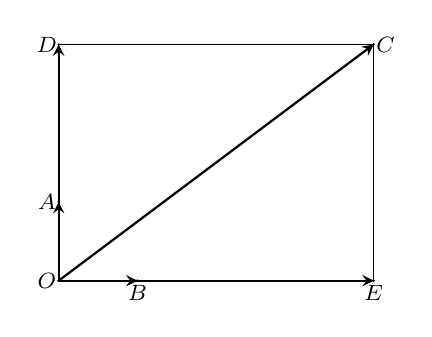
\begin{tikzpicture}[scale=0.5, font=\footnotesize, line join=round, line cap=round, >=stealth]
				\path	(0,0) coordinate (O)
				(2,0) coordinate (B)
				(0,2) coordinate (A)	
					(8,0) coordinate (E)
				(0,6) coordinate (D)	
					(8,6) coordinate (C)	;
				\draw[thick,->] (O)--(A);
				\draw[thick,->] (O)--(B);
				\draw[thick,->] (O)--(D);
				\draw[thick,->] (O)--(C);
					\draw[thick,->] (O)--(E);
				\draw (E)--(C)--(D);
				%\pic[draw,thin,angle radius=2mm] {right angle = D--A--B};
				%	\pic[draw,thin,angle radius=6mm,"$45$"] {angle = A--O--C};
				%	\pic[draw,thin,angle radius=6mm,"$45$"] {angle = D--O--A};
				\foreach \x/\g in {A/180,D/180,B/-90,E/-90,C/0,O/180}  \fill (\x) circle (1.0pt)+(\g:.3)node {$\x$};	
		\end{tikzpicture}}	
	}
\end{ex}


\begin{ex}%[text tai lieu Duong Hung, Huỳnh Xuân Tín]%[0H5V3-6]
	Cho tam giác $ABC$ đều có cạnh $AB=5$, $H$ là trung điểm của $BC$. Tính $\left|\overrightarrow{CA}-\overrightarrow{HC}\right|$.
	\choice
	{$\left|\overrightarrow{CA}-\overrightarrow{HC}\right|=\dfrac{5\sqrt{3}}{2}$}
	{$\left|\overrightarrow{CA}-\overrightarrow{HC}\right|=5$}
	{$\left|\overrightarrow{CA}-\overrightarrow{HC}\right|=\dfrac{5\sqrt{7}}{4}$}
	{\True $\left|\overrightarrow{CA}-\overrightarrow{HC}\right|=\dfrac{5\sqrt{7}}{2}$}
	\loigiai{
				\immini{	Ta có $\left|\overrightarrow{CA}-\overrightarrow{HC}\right|=\left|\overrightarrow{CA}+\overrightarrow{CH}\right|=\left|2\overrightarrow{CE}\right|=2CE$ (với $E$ là trung điểm của $AH$.\\
					Ta lại có $AH=\dfrac{5\sqrt{3}}{2}$ ($\triangle ABC$ đều, $AH$ là đường cao).\\
					Trong tam giác $HEC$ vuông tại $H$, có
					\[EC=\sqrt{CH^2+HE^2}=\sqrt{2.5^2+\left(\dfrac{5\sqrt{3}}{4} \right)^2}=\dfrac{5\sqrt{7}}{4} \Rightarrow \left|\overrightarrow{CA}-\overrightarrow{HC}\right|=2CE=\dfrac{5\sqrt{7}}{2}.
					\]}{\begin{tikzpicture}[scale=0.7, font=\footnotesize, line join=round, line cap=round, >=stealth]
					\path	(0,0) coordinate (A)
					(0:4) coordinate (B)
					(60:4) coordinate (C)	
					($(C)!0.5!(B)$) coordinate (H)
					($(H)!0.5!(A)$) coordinate (E);
					\draw[thick,->] (C)--(A);
					\draw[thick,->] (H)--(C);
					\draw[thick,->] (C)--(E);
					\draw (C)--(A)--(B)--(C) (A)--(H);
					\foreach \x/\g in {A/180,B/0,C/90,H/40,E/-90}  \fill (\x) circle (1.0pt)+(\g:.3)node {$\x$};	
			\end{tikzpicture}}	
		}
	\end{ex}



\begin{ex}%[text tai lieu Duong Hung, Huỳnh Xuân Tín]%[0H5V3-6]
	Cho $\triangle ABC$ đều cạnh $a$, gọi $H$ là trung điểm của cạnh $BC$. Tính $\left|\overrightarrow{CA}-\overrightarrow{HC}\right|$.
	\choice
	{\True $\dfrac{\sqrt{7} a}{2}$}
	{$\dfrac{a\sqrt{7}}{4}$}
	{$\dfrac{2\sqrt{3} a}{3}$}
	{$\dfrac{a}{2}$}
	\loigiai{
		\immini{	Gọi $D$ là điểm thỏa mãn $\overrightarrow{AD}=\overrightarrow{CH}$. Khi đó, $\left|\overrightarrow{CA}-\overrightarrow{HC}\right|=\left|\overrightarrow{CA}+\overrightarrow{CH}\right|=\left|\overrightarrow{CD}\right|=CD$.\\
			Ta thấy, $\overrightarrow{AD}=\overrightarrow{HB}$ vì $\overrightarrow{CH}=\overrightarrow{HB}$ (do $H$ trung điểm $BC$).\\		
			Suy ra, $AHBD$ là hình bình hành. Mà $AH\bot BC$ (vì $\triangle ABC$ đều). Vậy $AHBD$ là hình chữ nhật.\\
			Suy ra, $BD\bot BC$ và $BD=AH=\dfrac{a\sqrt{3}}{2}$.\\
			Áp dụng định lí Py-ta-go vào $\triangle DBC$ vuông tại $B$, có\\
			$$CD^2=BD^2+BC^2=\dfrac{3a^2}{4}+a^2=\dfrac{7a^2}{4} \Rightarrow CD=\dfrac{a\sqrt{7}}{2}.$$
		}{\begin{tikzpicture}[scale=0.7, font=\footnotesize, line join=round, line cap=round, >=stealth]
				\path	(0,0) coordinate (A)
				(0:4) coordinate (B)
				(60:4) coordinate (C)	
				(-60:2) coordinate (D)	
				($(C)!0.5!(B)$) coordinate (H)
				($(H)!0.5!(A)$) coordinate (E);
				\draw[thick,->] (C)--(A);
				\draw[thick,->] (H)--(C);
				\draw[thick,->] (H)--(B);
					\draw[thick,->] (A)--(D);
				\draw (C)--(A)--(B)--(C) (A)--(H) (B)--(D);
				\foreach \x/\g in {A/180,B/0,C/90,H/40,D/-90}  \fill (\x) circle (1.0pt)+(\g:.3)node {$\x$};	
		\end{tikzpicture}}	
\noindent 	
 Vậy $\left|\overrightarrow{CA}-\overrightarrow{HC}\right|=CD=\dfrac{a\sqrt{7}}{2}$.
	}
\end{ex}
\Closesolutionfile{ans}
\indapan{6}{ans/ans-0-B1}




\cauds
\Opensolutionfile{ans}[ans/ans-0-B1-DS]

%-------------------------------------------------------
\begin{ex}%[text tai lieu Duong Hung, Huỳnh Xuân Tín]%[0H5H3-2]
	%Câu 14.
	Cho tam giác $ABC$ có $G$ là trọng tâm. Gọi $M,N$ lần lượt là trung điểm của $AB,BC$. Lấy hai điểm $I,J$ sao cho: $2\overrightarrow{IA}+3\overrightarrow{IC}=\overrightarrow{0}$ và $2\overrightarrow{JA}+5\overrightarrow{JB}+3\overrightarrow{JC}=\overrightarrow{0}$. Các mệnh đề sau đúng hay sai?
	\choiceTF
	{\True $M$, $N$, $J$ thẳng hàng}
	{$\overrightarrow{JM}=\dfrac{3}{2}\overrightarrow{JN}$}
	{\True $J$ là trung điểm của $BI$}
	{\True Gọi $E$ là điểm thuộc $AB$ sao cho $\overrightarrow{AE}=\dfrac{5}{7}\overrightarrow{AB}$ thì $C$, $E$, $J$ thẳng hàng}
	\loigiai{
		\begin{center}
			\begin{tikzpicture}[scale=1.2, font=\footnotesize, line join=round, line cap=round, >=stealth]
				\path	(0,0) coordinate (A)
				(-1,-3) coordinate (B)
				($(B)+(4,0)$) coordinate (C)
				($(A)!1/2!(B)$)coordinate (M)
				($(B)!1/2!(C)$)coordinate (N)
				($(A)!2/3!(N)$)coordinate (G)
				($(A)!5/7!(B)$)coordinate (E)
				($(A)!3/5!(C)$)coordinate (I)
				(intersection of B--I and C--E)coordinate (J)
				;
				\draw (A)--(B)--(C)--cycle (B)--(I)(C)--(M) (C)--(E)(A)--(N);
				\foreach \x/\g in {A/90,B/-90,C/-90,I/20,N/-90,M/135,E/160,J/-90,G/50}  \fill (\x) circle (1.2pt)+(\g:.3)node[scale=0.8] {$\x$};	
			\end{tikzpicture}
		\end{center}
		\begin{itemchoice}
			\itemch Ta có  $2\overrightarrow{JA}+5\overrightarrow{JB}+3\overrightarrow{JC}=2(\overrightarrow{JA}+\overrightarrow{JB})+3(\overrightarrow{JB}+\overrightarrow{JC})=4\overrightarrow{JM}+6\overrightarrow{JN}=\overrightarrow{0}$
			$\Rightarrow \overrightarrow{JM}=-\dfrac{3}{2}\overrightarrow{JN}$. Do đó $J,M,N$ thẳng hàng.\\
			Điểm $J$ thuộc đoạn $MN$ và thỏa mãn $JM=\dfrac{3}{2}JN$.
			\itemch Ta có 
			\begin{eqnarray*}
				&& \overrightarrow{JM}=-\dfrac{3}{2}\overrightarrow{JN}\Leftrightarrow \overrightarrow{JM}=-\dfrac{3}{2}(\overrightarrow{JM}+\overrightarrow{MN})\\
				&\Leftrightarrow & \dfrac{5}{2}\overrightarrow{JM}=-\dfrac{3}{2}\overrightarrow{MN}\Leftrightarrow  \overrightarrow{JM}=-\dfrac{3}{5}\overrightarrow{MN}
					\end{eqnarray*}
			\itemch Ta có 
			\begin{eqnarray*}		
				&&2\overrightarrow{IA}+3\overrightarrow{IC}=\overrightarrow{0}\Leftrightarrow 2\overrightarrow{IC}+2\overrightarrow{CA}+3\overrightarrow{IC}=\overrightarrow{0}\Leftrightarrow \overrightarrow{CI}=\dfrac{2}{5}\overrightarrow{CA}.
			\end{eqnarray*}
			Khi đó: 
			\begin{eqnarray*}
				\overrightarrow{JB}&=&\overrightarrow{JM}+\overrightarrow{MB}=-\dfrac{3}{5}\overrightarrow{MN}+\dfrac{1}{2}\overrightarrow{AB}=-\dfrac{3}{10}\overrightarrow{AC}+\dfrac{1}{2}\overrightarrow{AB}\quad(1) \\
				\overrightarrow{BI}&=&\overrightarrow{BC}+\overrightarrow{CI}=\overrightarrow{BC}+\dfrac{2}{5}\overrightarrow{CA}=\overrightarrow{AC}-\overrightarrow{AB}-\dfrac{2}{5}\overrightarrow{AC}\\
				&=&\dfrac{3}{5}\overrightarrow{AC}-\overrightarrow{AB}=-2\left(-\dfrac{3}{10}\overrightarrow{AC}+\dfrac{1}{2}\overrightarrow{AB}\right)=-2\overrightarrow{JB}\text{ (do (1)).}
			\end{eqnarray*}
			Vậy $J$ là trung điểm của $BI$.
			\itemch \begin{eqnarray*}
				\overrightarrow{CJ}&=&\overrightarrow{CN}+\overrightarrow{NJ}\\
				&=&-\dfrac{1}{2}\overrightarrow{BC}+\dfrac{1}{2}\overrightarrow{CI}\\
				&=&-\dfrac{1}{2}\overrightarrow{BC}+\dfrac{1}{2}\cdot\dfrac{2}{5}\overrightarrow{CA}\\
				&=&-\dfrac{1}{2}(\overrightarrow{AC}-\overrightarrow{AB})-\dfrac{1}{5}\overrightarrow{AC}\\
				&=&-\dfrac{7}{10}\overrightarrow{AC}+\dfrac{1}{2}\overrightarrow{AB}.
			\end{eqnarray*} 
			Mặt khác:  $\overrightarrow{CE}=\overrightarrow{CA}+\overrightarrow{AE}=-\overrightarrow{AC}+k\overrightarrow{AB}$.\\
			Để $C,E,J$ thẳng hàng thì
			$$\begin{aligned}
			\exists m\in\; \mathbb{R},\overrightarrow{CE}=m\cdot\overrightarrow{CJ}&\Leftrightarrow -\overrightarrow{AC}+k\overrightarrow{AB}=-\dfrac{7m}{10}\overrightarrow{AC}+\dfrac{m}{2}\overrightarrow{AB}\\
			&\Leftrightarrow \heva{-1&=-\dfrac{7m}{10}\\
				k&=\dfrac{m}{2}}\Rightarrow \heva{m&=\dfrac{10}{7}\\k&=\dfrac{5}{7}}\Rightarrow k=\dfrac{5}{7}.
\end{aligned}			 
			$$
		\end{itemchoice}}
\end{ex}
%-------------------------------------------------------
\begin{ex}%[text tai lieu Duong Hung, Huỳnh Xuân Tín]%[0H5V3-2]
	%Câu 15. 
	Cho tứ giác $ABCD$. Gọi $I$, $J$ lần lượt là trung điểm $AB$ và $CD$, $K$ là trung điểm $IJ$, $M$ là điểm bất kì. Các mệnh đề sau đúng hay sai?
	\choiceTF
	{\True $\overrightarrow{AC}+\overrightarrow{BD}=2\overrightarrow{IJ}$}
	{\True $\overrightarrow{AD}+\overrightarrow{BC}=2\overrightarrow{IJ}$}
	{$\overrightarrow{MI}+\overrightarrow{MJ}=\overrightarrow{MK}$}
	{\True $\overrightarrow{MA}+\overrightarrow{MB}+\overrightarrow{MC}+\overrightarrow{MD}=4\overrightarrow{MK}$}
	\loigiai{
		\begin{itemchoice}
			\itemch $$\begin{aligned}
\overrightarrow{AC}+\overrightarrow{BD}&=\overrightarrow{AI}+\overrightarrow{IJ}+\overrightarrow{JC}+\overrightarrow{BI}+\overrightarrow{IJ}+\overrightarrow{JD}\\
			&=(\overrightarrow{AI}+\overrightarrow{BI})+2\overrightarrow{IJ}+(\overrightarrow{JC}+\overrightarrow{JD})=2\overrightarrow{IJ}.
\end{aligned}$$

			\itemch
$$\begin{aligned}
\overrightarrow{AD}+\overrightarrow{BC}&=\overrightarrow{AI}+\overrightarrow{IJ}+\overrightarrow{JD}+\overrightarrow{BI}+\overrightarrow{IJ}+\overrightarrow{JC}\\
			&=(\overrightarrow{AI}+\overrightarrow{BI})+2\overrightarrow{IJ}+(\overrightarrow{JD}+\overrightarrow{JC})=2\overrightarrow{IJ}.
\end{aligned}$$		
			 
			\itemch
$$\begin{aligned}
 \overrightarrow{AD}+\overrightarrow{BC}&=\overrightarrow{AI}+\overrightarrow{IJ}+\overrightarrow{JD}+\overrightarrow{BI}+\overrightarrow{IJ}+\overrightarrow{JC}\\
			&=(\overrightarrow{AI}+\overrightarrow{BI})+2\overrightarrow{IJ}+(\overrightarrow{JD}+\overrightarrow{JC})=2\overrightarrow{IJ}.
\end{aligned}$$			
			
			\itemch $\overrightarrow{MA}+\overrightarrow{MB}+\overrightarrow{MC}+\overrightarrow{MD}=2\overrightarrow{MI}+2\overrightarrow{MJ}=2(\overrightarrow{MI}+\overrightarrow{MJ})=4\overrightarrow{MK}$
		\end{itemchoice}}
\end{ex}
%-------------------------------------------------------
\begin{ex}%[text tai lieu Duong Hung, Huỳnh Xuân Tín]%[0H5V3-2]
	%Câu 16. 
	Cho tam giác $ABC$ có $M$ là trung điểm $BC$. Gọi $G$ là trọng tâm, $H$ là trực tâm, $O$ là tâm đường tròn ngoại tiếp tam giác $ABC,AA^\prime$ là đường kính của $(O)$. Các mệnh đề sau đúng hay sai?
	\choiceTF
	{\True $\overrightarrow{BH}=\overrightarrow{AC}$}
	{\True $\overrightarrow{AH}=2\overrightarrow{OM}$}
	{$\overrightarrow{HA}+\overrightarrow{HB}+\overrightarrow{HC}=3\overrightarrow{HO}$}
	{$\overrightarrow{OA}+\overrightarrow{OB}+\overrightarrow{OC}=3\overrightarrow{OH}$}
	\loigiai{
		\begin{center}
			\begin{tikzpicture}[scale=1, font=\footnotesize, line join=round, line cap=round, >=stealth]
				\path	(0,0) coordinate (A)
				(-1,-3) coordinate (B)
				($(B)+(4,0)$) coordinate (C)
				($(B)!1/2!(C)$)coordinate (M)
				($(A)!2/3!(M)$)coordinate (G)
				($(B)!(A)!(C)$)coordinate (a')
				($(A)!(C)!(B)$)coordinate (c')
				($(A)!(B)!(C)$)coordinate (b') 
				(intersection of A--a' and B--b')coordinate (H)
				($(H)!2!(M)$)coordinate (A')
				($(A)!1/2!(A')$)coordinate (O)
				;
				\draw (O) let \p1=($(O)-(A)$) in circle ({veclen(\x1,\y1)});
				\draw (A)--(B)--(C)--cycle (H)--(A')--(A)--(M)(A)--(a') (B)--(b') (C)--(c') (B)--(A')--(C);
				\foreach \x/\g in {A/90,B/-150,C/-45,M/-90,G/165,H/125,A'/-80,O/45}  \fill (\x) circle (1.2pt)+(\g:.35)node {$\x$};	
				\draw[fill] (M) circle (1pt) ($(A)!1/3!(M)$)circle (1pt);
			\end{tikzpicture}
		\end{center}
		\begin{itemchoice}
			\itemch Do tứ giác $BHCA^\prime$ có $BH\parallel A^\prime C(\perp AC)$ và $CH\parallel BA^\prime(\perp AB)$ nên $BHCA^\prime$ là hình bình hành
			$
			\Rightarrow \overrightarrow{BH}=\overrightarrow{A^\prime C}.$
			\itemch  Lại có $M$ là trung điểm của đường chéo $BC$ nên $M$ là trung điểm của $HA^\prime$ hay $H,M,A^\prime$ thẳng hàng.\\
			Do $OM$ là đường trung bình của $\triangle AHA^\prime$ nên $AH=2OM$, mà $\overrightarrow{AH}$ và $\overrightarrow{OM}$ cùng hướng
			$\Rightarrow \overrightarrow{AH}=2\overrightarrow{OM}.$
			\itemch $\overrightarrow{HA}+\overrightarrow{HB}+\overrightarrow{HC}=\overrightarrow{HA}+\overrightarrow{HA}$ (Tứ giác $AHCA$ là hình bình hành)\\
			$\overrightarrow{HA}=\overrightarrow{HB}+\overrightarrow{HC}=2\overrightarrow{HO}$
			\itemch
			\begin{eqnarray*}
\overrightarrow{OA}+\overrightarrow{OB}+\overrightarrow{OC}
				&=&\overrightarrow{OH}+\overrightarrow{HA}+\overrightarrow{OH}+\overrightarrow{HB}+\overrightarrow{OH}+\overrightarrow{HC}\\
				&=&3\overrightarrow{OH}+\overrightarrow{HA}+\overrightarrow{HB}+\overrightarrow{HC}\\
				&=&3\overrightarrow{OH}+2\overrightarrow{HO}=\overrightarrow{OH}.
			\end{eqnarray*}
		\end{itemchoice}}
\end{ex}
%-------------------------------------------------------
\begin{ex}%[text tai lieu Duong Hung, Huỳnh Xuân Tín]%[0H5V3-2]
	%Câu 17. 
	Cho hình bình hành $ABCD$. Gọi $I$, $J$ lần lượt là trung điểm $BC$ và $CD$. Các mệnh đề sau đúng hay sai?
	\choiceTF
	{\True $\overrightarrow{AC}=\overrightarrow{AB}+\overrightarrow{AD}$}
	{$\overrightarrow{AI}=\overrightarrow{AC}+\overrightarrow{AB}$}
	{$\overrightarrow{AI}=\overrightarrow{AB}+\dfrac{3}{2}\overrightarrow{AD}$}
	{$\overrightarrow{AJ}=\dfrac{1}{2}\overrightarrow{AB}+\dfrac{1}{2}\overrightarrow{AD}$}
	\loigiai{
		\immini{	\begin{itemchoice}
				\itemch $\overrightarrow{A C}=\overrightarrow{A B}+\overrightarrow{A D}$.
				\itemch $\overrightarrow{A I}=\dfrac{1}{2} \overrightarrow{A C}+\dfrac{1}{2} \overrightarrow{A B}$
				\itemch $\overrightarrow{A I}=\dfrac{1}{2}(\overrightarrow{A B}+\overrightarrow{A D})+\dfrac{1}{2} \overrightarrow{A B}= \overrightarrow{AB}+\dfrac{1}{2}\overrightarrow{AD}.$
				\itemch  $\overrightarrow{A J}=\dfrac{1}{2}(\overrightarrow{A D}+\overrightarrow{A C})=\dfrac{1}{2} \overrightarrow{A D}+\dfrac{1}{2}(\overrightarrow{A B}+\overrightarrow{A D})=\dfrac{1}{2} \overrightarrow{A B}+\overrightarrow{A D}$. 
			\end{itemchoice}}
		{\begin{tikzpicture}[scale=0.5, font=\footnotesize, line join=round, line cap=round, >=stealth]
				\path	(0,0) coordinate (A)
				(-2,-4) coordinate (B)
				($(B)+(6,0)$) coordinate (C)
				($(A)+(C)-(B)$)coordinate (D)
				($(C)!1/2!(B)$)coordinate (I)
				($(C)!1/2!(D)$)coordinate (J)
				;
				\draw (A)--(B)--(C)--(D)--cycle (I)--(A)--(C)(A)--(J);
				\foreach \x/\g in {A/90,B/-90,C/-90,D/90,I/-90,J/-30}  \fill (\x) circle (1.2pt)+(\g:.5)node {$\x$};	
		\end{tikzpicture}}
	}
\end{ex}


\Closesolutionfile{ans}
\indapan{3}{ans/ans-0-B1-DS}



\Opensolutionfile{ans}[ans/ans-0-B1-KQ]
\caukq
%%%==============BT_14==============%%%
\begin{ex}%[text tai lieu Duong Hung, Huỳnh Xuân Tín]%[0H5H3-5]
	Cho $4$ điểm $A$, $B$, $C$, $D$. Gọi $I$, $J$ lần lượt là trung điểm của $B C$ và $C D$. Khi đó $\overrightarrow{AB}+\overrightarrow{A I}+\overrightarrow{J A}+\overrightarrow{D A}=k \overrightarrow{D B}$. Vậy $k$ bằng bao nhiêu?\par
	\shortans{$1{,}5$}
	\loigiai
	{
		Ta có 
		\begin{eqnarray*}
			\overrightarrow{AB}+\overrightarrow{A I}+\overrightarrow{J A}+\overrightarrow{D A}&=&\overrightarrow{D A}+\overrightarrow{AB}+\overrightarrow{J A}+\overrightarrow{A I} \\
			&= & \overrightarrow{D B}+\overrightarrow{I J}\\
			&= & \overrightarrow{D B}+\overrightarrow{J I}\\
			&=& \overrightarrow{D B}+\dfrac{1}{2} \overrightarrow{D B}\\
			&=& \dfrac{3}{2} \overrightarrow{D B}.
		\end{eqnarray*}
	}
\end{ex}
%%%==============BT_15==============%%%
\begin{ex}%[text tai lieu Duong Hung, Huỳnh Xuân Tín]%[0H5H3-5]
	Cho $\triangle A B C$. Gọi $J$ là điểm trên cạnh $A C$ sao cho $J A=\dfrac{2}{3} J C$. Nếu $\overrightarrow{BJ}=m\overrightarrow{BA}+n\overrightarrow{B C}$ thì giá trị $m+n$ bằng bao nhiêu?
	\shortans{$1$}
	\loigiai{
		Ta có $JA=\dfrac{2}{3} J C \Leftrightarrow  3 JA =2 JC$. Mà $\overrightarrow{JA}$ và $\overrightarrow{JC}$ ngược hướng, nên
		\begin{eqnarray*}
			3 JA =2 JC&\Leftrightarrow & 3 \overrightarrow{J A}=-2 \overrightarrow{J C}\\
			&\Leftrightarrow & 3\left(\overrightarrow{B A}-\overrightarrow{B J}\right)+2\left(\overrightarrow{B C}-\overrightarrow{B J}\right)=\overrightarrow{0}\\
			&\Leftrightarrow & 5 \overrightarrow{B J}=3 \overrightarrow{B A}+2 \overrightarrow{B C}\\
			&\Leftrightarrow & \overrightarrow{B J}=\dfrac{3}{5} \overrightarrow{B A}+\dfrac{2}{5} \overrightarrow{BC}.
		\end{eqnarray*}
		Khi đó $m+n=1$.
	}
\end{ex}

\begin{ex}%[text tai lieu Duong Hung, Huỳnh Xuân Tín]%[0H5H3-1]
	Cho $\triangle A B C$ có điểm $D$, $I$ thỏa $3 \overrightarrow{DB}=2 \overrightarrow{D C}$, $\overrightarrow{I A}+3 \overrightarrow{I B}-2 \overrightarrow{I C}=\overrightarrow{0}$. Nếu $\overrightarrow{A D}=k \overrightarrow{A I}$ thì $k$ bằng bao nhiêu?
	\shortans{$2$}
	\loigiai{
		Ta có 
		\begin{eqnarray*}
			& & \overrightarrow{IA}+3 \overrightarrow{IB}-2 \overrightarrow{IC}=\overrightarrow{0}\\
			&\Leftrightarrow & -\overrightarrow{AI}+3\left(\overrightarrow{AB}-\overrightarrow{AI}\right)-2\left(\overrightarrow{AC}-\overrightarrow{AI}\right)=\overrightarrow{0}\\
			&\Leftrightarrow & -\overrightarrow{AI}+3 \overrightarrow{AB}-3 \overrightarrow{A I}-2 \overrightarrow{AC}+2 \overrightarrow{AI}=\overrightarrow{0}\\
			&\Leftrightarrow & 2 \overrightarrow{AI}=3\overrightarrow{AB}-2 \overrightarrow{AC}\\
			&\Leftrightarrow & \overrightarrow{AI}=\dfrac{3}{2} \overrightarrow{AB}-\overrightarrow{AC}.
		\end{eqnarray*}
		Ta lại có 
		\begin{eqnarray*}
			& & 3\overrightarrow{DB}=2 \overrightarrow{DC}\\
			&\Leftrightarrow & 3\left(\overrightarrow{AB}-\overrightarrow{A D}\right)=2\left(\overrightarrow{AC}-\overrightarrow{AD}\right)\\
			&\Leftrightarrow & 3\overrightarrow{AB}-3\overrightarrow{AD}=2\overrightarrow{AC}-2\overrightarrow{AD}\\
			&\Leftrightarrow &\overrightarrow{AD}=3 \overrightarrow{AB}-2\overrightarrow{AC}.
		\end{eqnarray*}
		Khi đó
		$\heva{&\overrightarrow{A I}=\dfrac{3}{2}\overrightarrow{AB}-\overrightarrow{AC} \\ &\overrightarrow{AD}=3\overrightarrow{AB}-2\overrightarrow{AC}} \Leftrightarrow \heva{&2 \overrightarrow{AI}=3\overrightarrow{AB}-2\overrightarrow{AC} \\ &\overrightarrow{AD}=3\overrightarrow{AB}-2 \overrightarrow{AC}} \Leftrightarrow \overrightarrow{AD}=2 \overrightarrow{A I}$.
	}
\end{ex}

\begin{ex}%[text tai lieu Duong Hung, Huỳnh Xuân Tín]%[0H5H3-7]
	Cho tam giác $ABC$. Gọi $G$ là trọng tâm của $\triangle ABC$. Cho điểm $M$ sao cho $\left|\overrightarrow{MA}+\overrightarrow{MB}+\overrightarrow{MC}\right|=6$, khi đó điểm $M$ thuộc đường tròn có bán kính bằng bao nhiêu?	\par
	\shortans{$2$}
	\loigiai{
		Ta có $\overrightarrow{MA}+\overrightarrow{MB}+\overrightarrow{MC}=3 \overrightarrow{M G}\Rightarrow \left|\overrightarrow{MA}+\overrightarrow{MB}+\overrightarrow{MC}\right|=3\left|\overrightarrow{M G}\right|=3 M G \Leftrightarrow M G=2$.\\
		Vậy tập hợp điểm $M$ là đường tròn tâm $G$ bán kính bằng $2$.
	}
\end{ex}
%%%==============BT_20==============%%%
\begin{ex}%[text tai lieu Duong Hung, Huỳnh Xuân Tín]%[0H5H3-1]%Câu 4
	Cho hình bình hành $ABCD$. Trên các đoạn thẳng $DC$, $AB$ theo thứ tự lấy các điểm $M$, $N$ sao cho $DM=BN$. Gọi $P$ là giao điểm của $AM$, $DB$ và $Q$ là giao điểm của $CN$, $DB$. Nếu $\overrightarrow{DB}=k \overrightarrow{Q B}$ thì $k$ bằng bao nhiêu?
	\shortans{$1$}
	\loigiai{
		Ta có $DM=BN \Rightarrow AN=MC$, mặt khác $AN$ song song với $MC$ do đó tứ giác $ANCM$ là hình bình hành Suy ra $\overrightarrow{AM}=\overrightarrow{NC}$.\\
		Xét tam giác $\triangle DMP$ và $\triangle BNQ$ ta có $DM=NB$ (giả thiết), $\widehat{PDM}=\widehat{QBN}$ (so le trong).\\
		Mặt khác $\widehat{D M P}=\widehat{A P B}$ (đối đỉnh) và $\widehat{A P Q}=\widehat{N Q B}$ (hai góc đồng vị) suy ra $\widehat{D M P}=\widehat{B N Q}$.\\
		Do đó $\triangle DMP=\triangle BNQ$ (c.g.c) suy ra $DB=QB$.\\
		Dễ thấy $\overrightarrow{DB}$, $\overrightarrow{QB}$ cùng hướng vì vậy $\overrightarrow{DB}=\overrightarrow{QB}$.
	}
\end{ex}
%%%==============BT_21==============%%%
\begin{ex}%[text tai lieu Duong Hung, Huỳnh Xuân Tín]%[0H5H3-1]%Câu 5
	Cho tam giác $ABC$. Trên cạnh $AB$ lấy điểm $M$ sao cho $2BA=5BM$. Gọi $G$ là trọng tâm tam giác $ABC$. Gọi $N$ là điểm trên $AC$ sao cho $AN=xAC$. Tìm $x$, biết ba điểm $M$, $N$, $G$ thẳng hàng. 
	\shortans{$0{,}75$}
	\loigiai{
		Ta có
		\begin{itemize}
			\item $\overrightarrow{MG}=\overrightarrow{AG}-\overrightarrow{AM}=\dfrac{1}{3}\left(\overrightarrow{AB}+\overrightarrow{AC}\right)-\dfrac{3}{5}\overrightarrow{AB}=\dfrac{1}{3}\overrightarrow{A C}-\dfrac{4}{15}\overrightarrow{AB}$.
			\item $\overrightarrow{MN}=\overrightarrow{AN}-\overrightarrow{AM}=x \overrightarrow{AC}-\dfrac{3}{5}\overrightarrow{AB}$.
		\end{itemize}
		Do $M$, $N$, $G$ thẳng hàng nên	$\overrightarrow{MN}=k \overrightarrow{MG}\Rightarrow \dfrac{x}{\dfrac{1}{3}}=\dfrac{-\dfrac{3}{5}}{-\dfrac{4}{15}}\Rightarrow 3 x=\dfrac{9}{4}\Rightarrow x=\dfrac{3}{4}$.
	}
\end{ex}
\Closesolutionfile{ans}
\indapan{6}{ans/ans-0-B1-KQ}




